%   Include in future work or lander or wherever
%   target 2-4 pages
\autsection{Ice Sounder and Penetrator Tracking Radar}{Gustavo Feijóo Carrillo}
%   main goal: provide penetrator tracking, depth

As future study, a promising method for positioning and tracking the penetrator as it makes its descent through the ice crust would to employ an ice sounder from the surface looking down in the direction of the descent path. Acquiring  the most accurate position for the penetrator becomes increasingly relevant as it comes closer to the ocean/ice interface where the inhomogeneity of the ice crust poses a risk for the mission and makes it critical to determine the depth at which the penetrator shall anchor itself. This ranging of the penetrator is also useful during the long period of melting through where this telemetry data may become relevant for unforseen events during the descent, like helping avoid obstacles in the path of the penetrator that an the on-board proximity sensors can't handle. 

%\begin{figure}[htb]
%	\centering
%	\includegraphics[width=.8\textwidth]{figures/iRadar/pDepth-EuropaIce.gif}
%	\caption{Penetration depth for RF in ice at different temperatures.}
%	\label{fig:iceRadar-pdepth}
%\end{figure}

Range resolution for an frequency modulated pulse radar is given by
\begin{equation}
    \Delta R = \frac{c}{2B}
\end{equation}
where $B$ is the bandwidth of the pulse modulation.

\begin{figure}[htb]
	\centering
	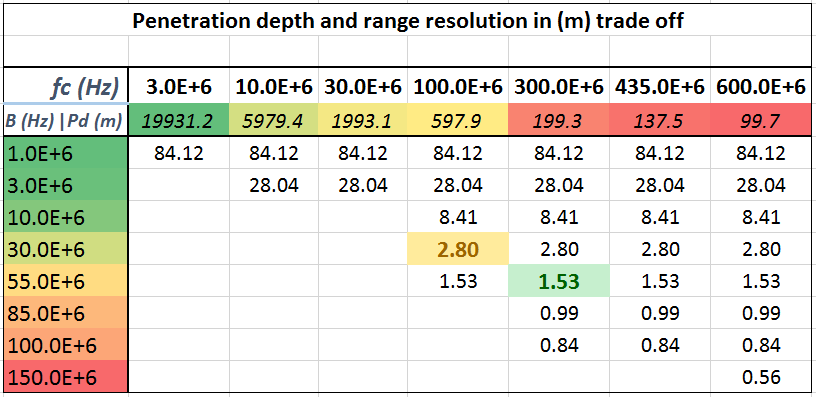
\includegraphics[width=.66\textwidth]{figures/iRadar/iceRadar-res-trade}
	\caption{Trade off between carrier frequency for penetration depth and pulse bandwidth which determines range resolution of the radar.}
	\label{fig:iceRadar-res-trade}
\end{figure}

From this brief example we can say that choice of resolution is possible in relevance to the dimension of the penetrator itself.